% 20200815
\documentclass[../thesis.tex]{subfiles} %% use packages & commands as this main file
\begin{document}

\subsection{The model}
The system was a set of ordinary differential equations (ODE).  It was a temperature-independent system with two biological components (\phy\ and \bac) and three density state variables (organic carbon $C$, \phy\ biomass $P$ and \bac l biomass $B$). \Phy\ and \bac\ received carbon from different sources but performed the same functions (Fig.\ref{f:model}). \Phy\ photosynthesized carbon dioxide from the atmosphere (an unlimited source) and \bac\ consumed carbon from the $C$ pool.  Both \phy\ and \bac\ had three ways to allocate carbon: respiration, leakage and biomass incorporation. Some biomass from each component died and became carbon in the $C$ pool.  Organic carbon in the environment could either be consumed by \bac\ or harvested but not reabsorbed by \phy.  Four major assumptions were upheld:  \Rn{1}) environmental conditions were always spatially homogeneous; \Rn{2}) unlimited nutrient; \Rn{3}) light intensity was homogeneous in the whole system as the culture could be shaped as a thin panel; \Rn{4}) \bac\ had no preference on any carbon types in the $C$ pool.  In short, living space for \phy\ was the only limiting factor.

The rate of carbon density change of state variables (grams of carbon per metre cube per day, \dxdt) were the currencies in our equations.  The equations were composed of three state variables of carbon densities, four life history traits of \phy, four life history traits of \bac\ and one harvest rate parameter (Eq.\ref{eq:PBH}).

\begin{equation}\left\{\begin{array}{rl}
    C'(t) &= \ePR(1-\eP)\cdot\gP\cdot P +\aP\cdot P^2 +(\eBR(1-\eB)-1)\cdot\gB\cdot C\cdot B +\mB\cdot B -xC\\
    P'(t) &= \ePR\cdot\eP\cdot\gP\cdot P -\aP\cdot P^2\\
    B'(t) &= \eBR\cdot\eB\cdot\gB\cdot C\cdot B -\mB\cdot B
\end{array}\right.\label{eq:PBH}\end{equation}

In Eq.\ref{eq:PBH}, $C'(t)$, $P'(t)$ and $B'(t)$ were the rates of density change (\dxdt).  $\ePR$ was the fraction of non-respired carbon for $P$, $\eP$ was the fraction of carbon incorporated as $P$ biomass, $\eBR$ was the fraction of non-respired carbon for $B$ and $\eB$ was the fraction of carbon incorporated as $B$ biomass.  These four were ``fraction parameters”.  $\gP$ was the growth rate of $P$ (\dayU), $\aP$ was the intraspecific interference of $P$ (\denI), $\gB$ was the resource clearance rate of $B$  (\denI) and $\mB$ was the death rate of $B$ (\dayU).  These four were ``rate parameters”.  $x$ was the harvest rate (\dayU), which was the speed of carbon harvest from the $C$ pool in a continuous harvest system.  $x$ was set to zero in destructive harvest systems and the harvest interval $T$ (day) was the replacement parameter.  The interval was defined as

\begin{equation}
    T = x-1
    \label{eq:TvsX}
\end{equation}

Values of equivalent $T$ and $x$ were differ by 1 because the day of system establishment was day 0.  Continuous harvest started on day 0 but destructive harvest started on day 1.  Carbon yield from continuous harvest on the very first day was equivalent to the carbon harvested by destructive harvest on the second day.

Daily yield in continuous harvest systems was defined as

\begin{equation}
    \text{daily yield} = x\cdot C
    \label{eq:yield}
\end{equation}

and the equivalent for destructive harvest was ``average yield", which was defined as

\begin{equation}
    \text{average yield} = \dfrac{[\text{total carbon}]|_{T}-[\text{total carbon}]|_{T=0}}{T}
    \label{eq:avgYd}
\end{equation}

\begin{figure}[H]
    \centering
    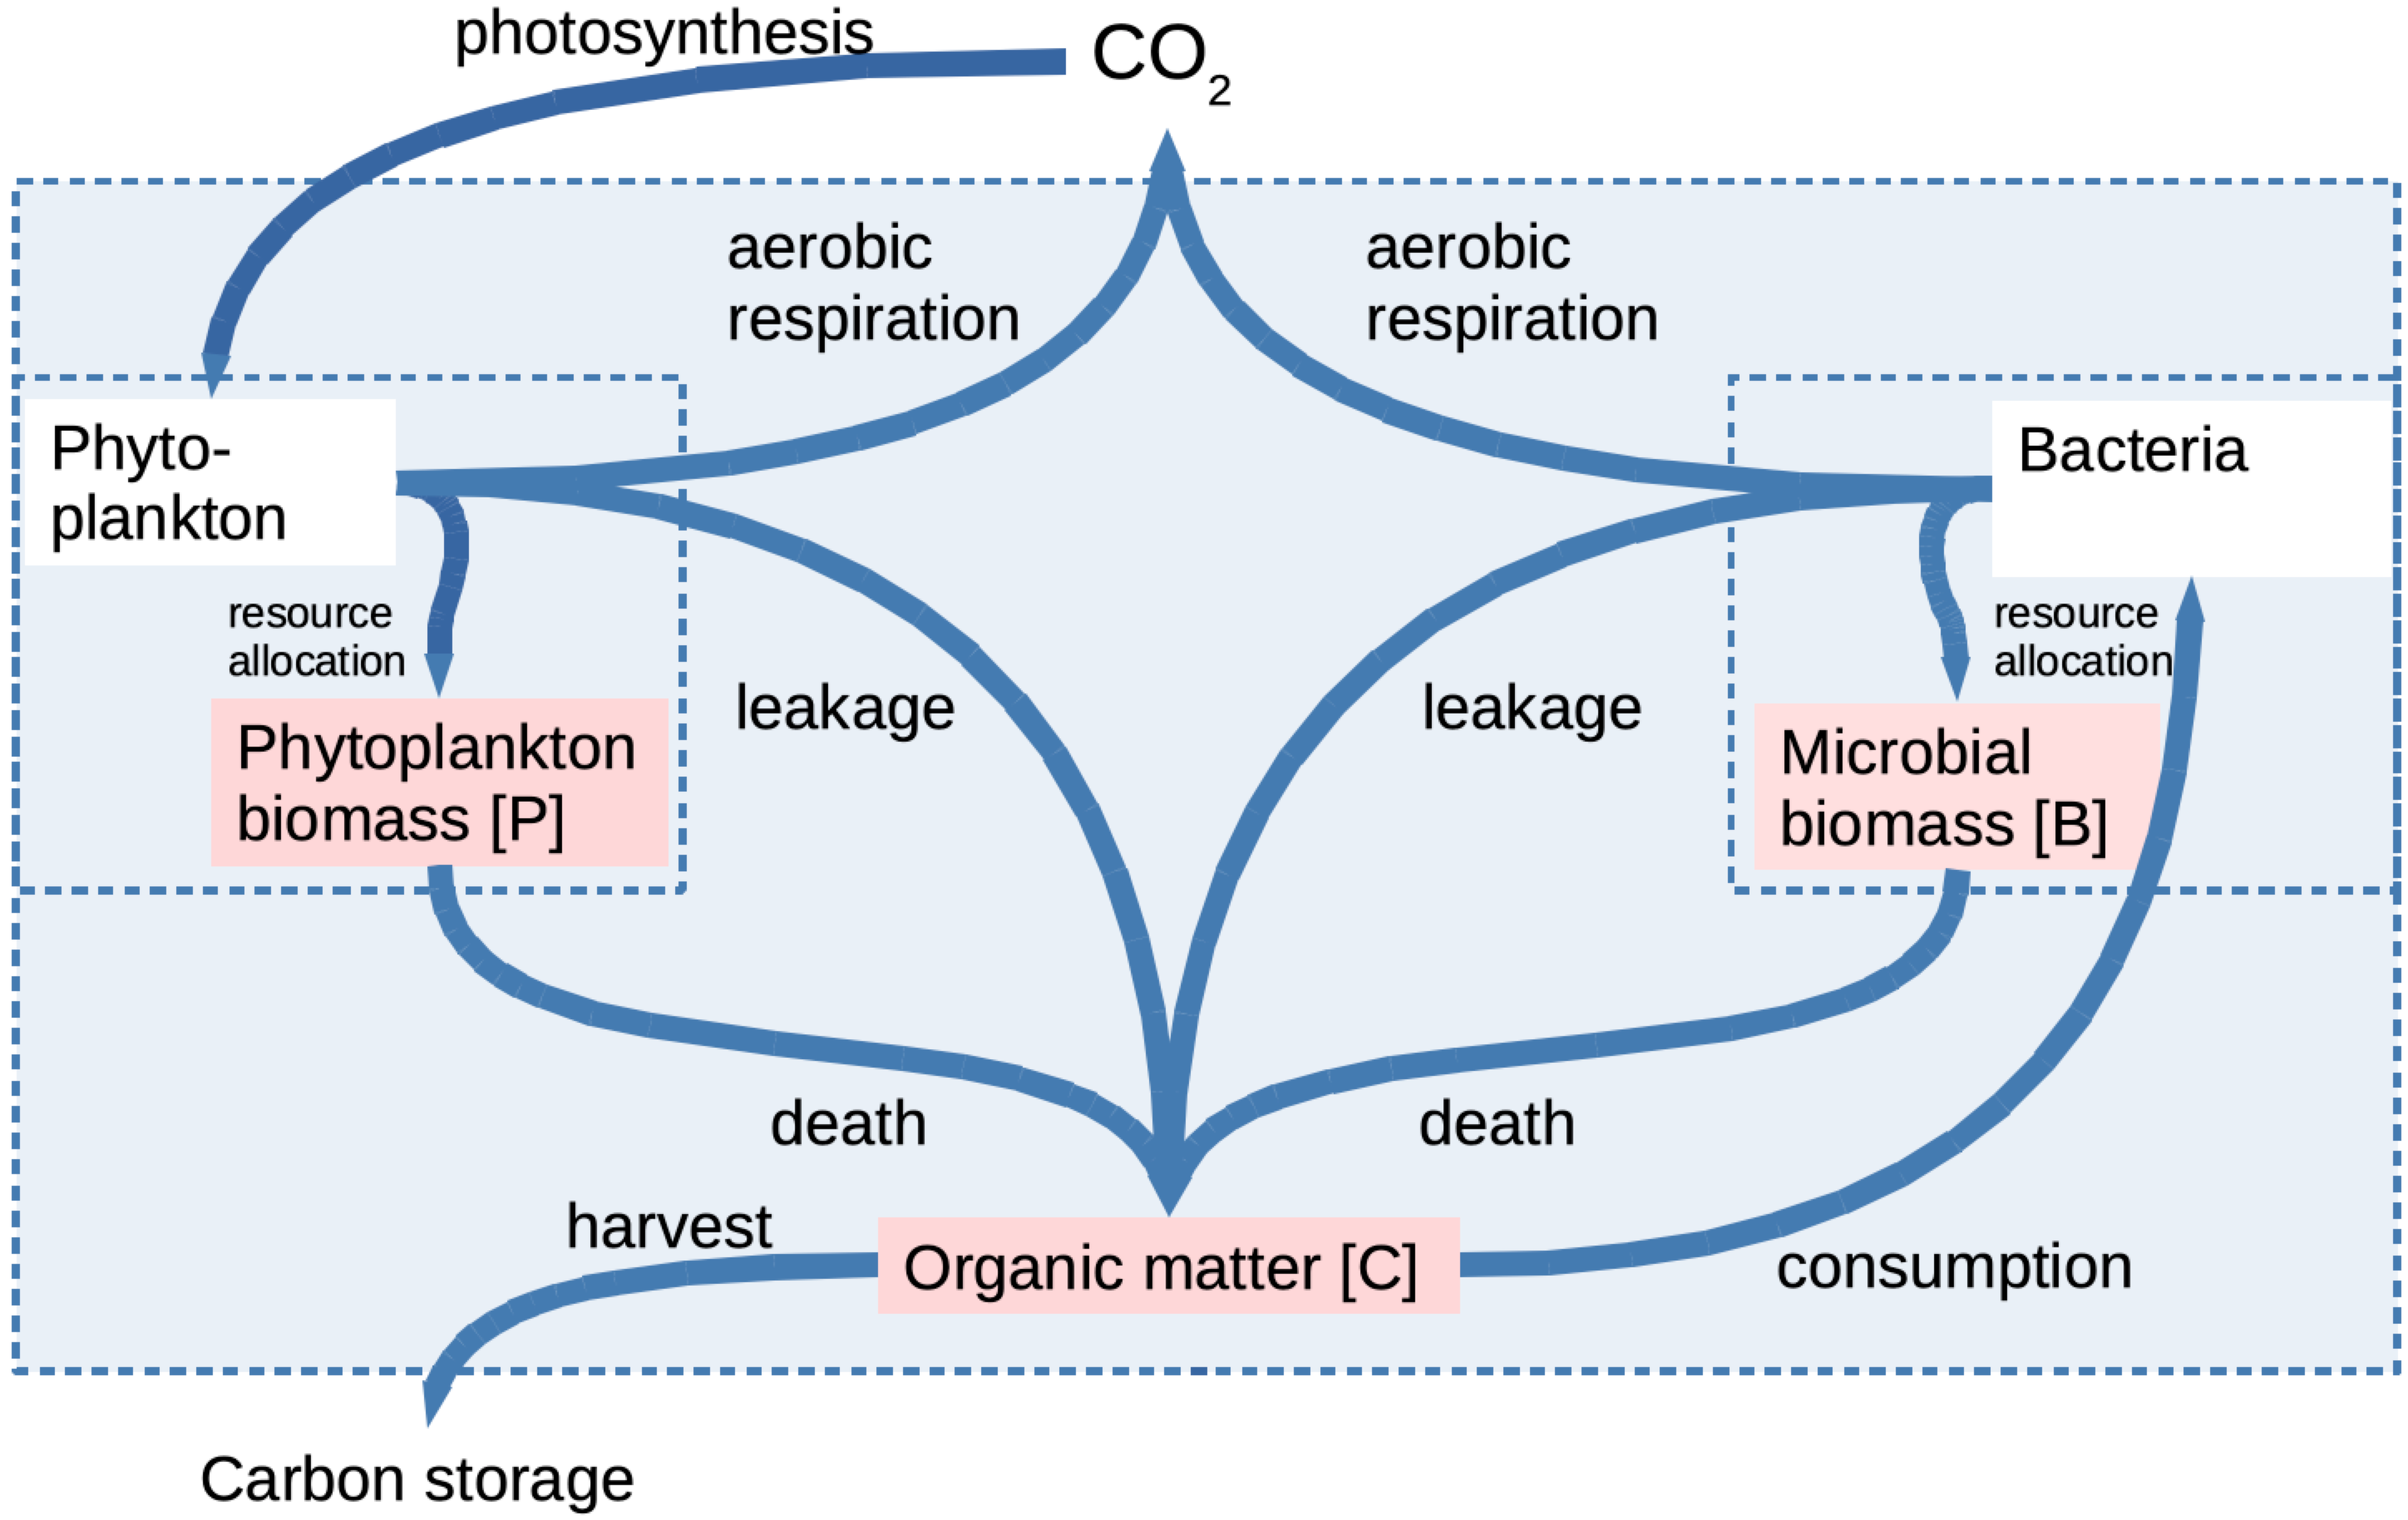
\includegraphics[width=.8\linewidth]{media/model.png}
    \caption[Model visualization]{The theoretical coexistence open system of \phy\ and \bac\ allows carbon exchange with external carbon dioxide source.  The dashed box is the defined boundary allowed matter exchange.  Blue arrows are the directions of carbon flow.  Pink boxes are the carbon pools (i.e. state variables).  White boxes are biochemical processes in indicated organisms.  These processes diverge carbon from source to different carbon pools.}
    \label{f:model}
\end{figure}

Eq.\ref{eq:PBH} was a \pbs\ of $P$ and $B$ under continuous harvest (\PBH).  Three alternative versions on $P$-only continuous harvest (\PoH), $P$ and $B$ destructive harvest (\PBN) and $P$-only destructive harvest (\PoN) were branched.

Continuous harvest \phy-only system (\PoH);
\begin{equation}\left\{\begin{array}{rl}
    C'(t) &= \ePR(1-\eP)\cdot\gP\cdot P +\aP\cdot P^2 -xC\\
    P'(t) &= \ePR\cdot\eP\cdot\gP\cdot P -\aP\cdot P^2
\end{array}\right.\label{eq:PoH}\end{equation}

Destructive harvest \pbs\ of $P$ and $B$ (\PBN); and
\begin{equation}\left\{\begin{array}{rl}
    C'(t) &= \ePR(1-\eP)\cdot\gP\cdot P +\aP\cdot P^2 +(\eBR(1-\eB)-1)\cdot\gB\cdot C\cdot B +\mB\cdot B\\
    P'(t) &= \ePR\cdot\eP\cdot\gP\cdot P -\aP\cdot P^2\\
    B'(t) &= \eBR\cdot\eB\cdot\gB\cdot C\cdot B -\mB\cdot B
\end{array}\right.\label{eq:PBN}\end{equation}

Destructive harvest \phy-only system (\PoN).
\begin{equation}\left\{\begin{array}{rl}
    C'(t) &= \ePR(1-\eP)\cdot\gP\cdot P +\aP\cdot P^2\\
    P'(t) &= \ePR\cdot\eP\cdot\gP\cdot P -\aP\cdot P^2
\end{array}\right.\label{eq:PoN}\end{equation}

Three biologically meaningful system stable states for continuous harvest systems were deduced using SymPy (v1.5.1) in python3 (v3.7.3) (Table \ref{t:eqm}).  Equilibrium 2 \& 3 were \PoH\ \& \PBH\ respectively with equilibrium 1 as a common alternative stable state.  Destructive systems could only be investigated through integration because the analytical solutions were the state variables.

\begin{table}[H]
    \centering
    \caption[Model equilibria]{Equilibria from the four variations of the proposed model (Eq.\ref{eq:PBH})}
    \begin{tabular}{cl|ccc}\hline
        equilibrium & scenario & $C$ & $P$ & $B$ (\PBH\ only) \\\hline
        1 & \PBH, \PoH & 0 & 0 & 0 \\
        2 & \PBH, \PoH & $\dfrac{\eP(\ePR\gP)^2}{\aP x}$ & $\dfrac{\ePR\eP\gP}{\aP}$ & 0 \\
        3 & \PBH & $\dfrac{\mB}{\eBR\eB\gB}$ & $\dfrac{\ePR\eP\gP}{\aP}$ & $\dfrac{(\ePR\gP)^2\eBR\eB\gB-\aP\mB x}{(1-\eBR)\aP\gB\mB}$ \\\hline
    \end{tabular}
    \label{t:eqm}
\end{table}

\subsection{Parameter space}
Data of the defined parameters in Eq.\ref{eq:PBH} was collected from literature.  Data was temperature-standardized to \temp\ because most available data was in this temperature range.  Parameters less than five data points were called ``data deficient".  Half of the above defined parameters were data deficient.  The widest percentage range in respective parameter groups was inferred as the logical range for these data-deficient parameters.  The selection was based on the Metabolic Theory of Ecology \autocite{brown2004toward}, which suggested that similar body size organisms shared similar metabolic rate.  Similar life history traits for unicellular organisms, \phy\ and \bac, therefore would potentially share similar parameter ranges because they were similar in cell size.  From the defined ranges (Table \ref{t:ranges}), 11 evenly-spaced sample values was selected to form the parameter space for the model.  The methods of determining each biological parameter range were in the appendix (section 10.2-10.9).

\begin{table}[H]
    \centering
    \caption[Algebra variables]{Biological variables and corresponding ranges framing the parameter space}
    \begin{tabular}{cclll}\hline
        variable & unit & description & min & max \\\hline
        $N'(t)$ & \dxdt & rate of change of respective carbon pool {\tiny($N=C,P,B$)} & - & - \\
        $N$ & \den & carbon density for respective pool {\tiny($N=C,P,B$)} & - & - \\
        $\ePR$ & - & non-respired carbon fraction for $P$ & 0.08 & 0.87 \\
        $\eP$ & - & assimilated carbon fraction for $P$ & 0.40 & 1.00 \\
        $\gP$ & \dayU & growth rate of $P$ & 0.03 & 3.17 \\
        $\aP$ & \denI & intraspecific interference of $P$ & 0.02 & 1.52 \\
        $\eBR$ & - & non-respired carbon fraction for $B$ & 0.13 & 1.00 \\
        $\eB$ & - & assimilated carbon fraction for $B$ & 0.07 & 0.82 \\
        $\gB$ & \denI & clearance rate of $B$ & 0.10 & 3.50 \\
        $\mB$ & \dayU & death rate of $B$ & 0.01 & 0.63 \\
    \hline\end{tabular}
    \label{t:ranges}
\end{table}

\subsection{Scenario sampling}
A set of 5500 (11 sample values $\times$ 500 expected sample frequency) unique biological parameter combinations were randomly selected via a uniform prior with seed number ``20192020" in R (v4.0.2).  This Latin Hypercube Sampling (LHS) method was to ensure the widest parameter space covered with a limited sample size.  200 evenly-spaced harvest rates ($x$) ranged 1-19901 \dayU were applied on each set of combinations on continuous harvest systems.  An equivalent harvest interval samples ($T$ = 0-19900 days, 200 evenly-spaced samples) were applied for each set of combinations on destructive harvest systems.

\subsection{Model experiment}
Continuous harvest system carbon contents were analytically calculated by C-lang (compiler gcc v7.5.0) using equilibrium positions from Table \ref{t:eqm}. Yield in \PoH\ was independent from harvest rates as defined in Eq.\ref{eq:yield}.  Destructive harvest system carbon contents were numerically integrated by python3 (v3.7.3) SciPy (v1.2.3) ``odeint" function using Eq.\ref{eq:PBH}.  Initial densities for \PBN\ and \PoN\ were $C=P=B=1$ and $C=P=1$, $B=0$ \den\ respectively.  I also integrated destructive systems in a log-spaced time ($T$ = 0-100) to observe the system behaviour before stability.

\subsection{Carbon yield analysis}
Feasible solutions were defined as all state variables in respective parameter combination were non-negatives.  Unfeasible solutions were set as invalid data (NA) for observing yield distributions within feasibility limits.  The data was right-skewed with outlier values more than 100x of the median in its respective set.  Pairwise Wilcox signed rank tests in R (v4.0.2) with bonferroni adjustment and no paired situations were therefore chosen for median comparisons between systems.  Early destructive systems development were plotted on log-spaced time.  Effect of \bac\ was compared within each harvest mode on selected harvest intervals/rates.  Effect of biological parameters were deduced through log-yield distributions across each parameter.

\end{document}